
\section{Aplicacions}

Els radio altímetres són uns components essencials per l'aeronavegació doncs proporcionen informació útil per l'execució de diverses operacions que garanteixen la seguretat de les aeronaus. Aquestes operacions són les següents:

\textbf{Sistemes automàtics de control de vol}

Els sistemes de control de vol de les aeronaus depenen de la informació d'alçada proporcionada pels radio altímetres a bord per tal de conèixer en tot moment la distància absoluta de les aeronaus respecte el terreny i així poder garantir la seguretat amb la seva correcte actuació.

\textbf{Aproximació i aterratge d'aeronaus}

Durant la fase d'aproximació d'una aeronau el radio altímetre, juntament amb altres sistemes mesuradors de distancia i sistemes d'aterratge, proporciona informació d'altitud respecte a terra de l'aeronau que els sistemes de control de vol d'abord utilitzen per ajustar l'aeronau als paràmetres establerts d'aterratge. Arribats a una certa alçada, al iniciar-se la fase d'aterratge els radio altímetres són els únics components proporcionant mesures d'alçada vertical que son utilitzades pel sistema d'autopilot per efectuar l'aterratge.  

Si el sistema de radio altímetres d'una aeronau no funciona o proporciona dades errònies les conseqüències van des de la necessitat de realitzar un aterratge manual en visual (sense autopilot) si l'aeroport ho permet i la visibilitat és bona, a la necessitat de desviar-se a una aeroport proper que ho permeti que sí ho permeti. 

\textbf{Sistema d'alerta de proximitat al sòl}

El sistema d'alerta de proximitat al sòl a bord de les aeronaus està dissenyat per evitar col·lisions així com evitar l'excessiu apropament de l'aeronau a obstacles situats sota aquesta garantint la seva seguretat. Per fer-ho proporciona de manera automàtica avisos de proximitat de terreny sota l'aeronau a la tripulació.  

Els diferents tipus o modes d'avisos proporcionats per aquest sistema són el següents:
\begin{multicols}{2}
\begin{itemize}
\item Rati de descens elevat
\item Rati d'aproximació a terra excessiu
\item Pèrdua d'altitud durant enlairament
\item Espai no segur per proximitat a terra
\item Desviació excessiva respecta la \textit{senda de planeo}
\end{itemize}
\end{multicols}
Com es pot apreciar, tots aquest avisos estan basats en l'altitud de l'aeronau respecte el sòl a sota d'aquesta i per tant depenen de la informació proporcionada pels radio altímetres. 


\section{Models Comercials}

En aquesta secció és presenta un model comercial típic de radio altímetre juntament amb les seves especificacions.

\textbf{Radio Altimetre RA 4000$/$4500}

	\begin{figure}[H]
	\centering
	  \begin{subfigure}[b]{0.32\textwidth}
	  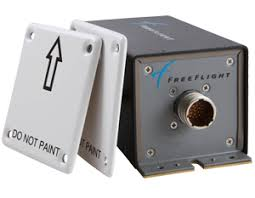
\includegraphics[width=\textwidth]{./images/RA4000.png}
	  \caption{}
	  \label{1diag1}
	  \end{subfigure}
	  \qquad %~ %add desired spacing between  images, e. g. ~, \quad,  \qquad, \hfill etc. 
	  \begin{subfigure}[b]{0.4\textwidth}
	  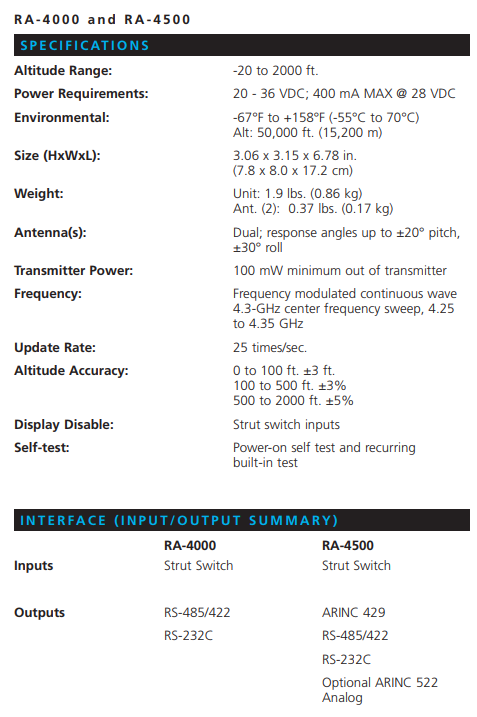
\includegraphics[width=\textwidth]{./images/RA4000Specs.png}
	  \caption{}
	  \label{1diag2}
	  \end{subfigure}
	  \vspace{10pt}
	\caption{Radio Altimetre RA 4000$/$4500 \cite{Systems}}
	\label{diag1}
	\end{figure}
